\section{Results}
\label{sec:results}

Despite the effort made in the implementation of the SCGS and SIMPLE algorithms, the results are not satisfactory.

Both the SIMPLE and SCGS are not stable and quickly diverge if the following conditions are met:

\begin{itemize}
    \item Too high under relaxation factors are chosen (>0.1)
    \item High Reynolds number (>100)
    \item Coarse mesh
\end{itemize}

The combination of the above conditions leads to a divergence of the solution.

For SCGS the problem can be spotted as a non-diagonal dominance of Vanka's matrix.

For SIMPLE, an analysis of the residual between iteration, shows that the code starts converging (up to $~200$ outer iterations) and the solution of the problem seems reasonable.
Suddenly some issue in the corner top-right of the domain brings to a rapid divergence of the system.

At this point we believe that the issue is somewhere in the coefficients used for convection, and in particular about the computation of fluxes.
However, after several attempts, we were not able to spot the issue.


\subsection{Results for the Lid-Driven Cavity Flow}

Here we present the results for the Lid-Driven Cavity Flow, computed using both the SCGS and SIMPLE algorithms.

In Figure \ref{fig:ghia_solution}, we leave our reference for the solution of the Lid-Driven Cavity Flow, as computed by \cite{Ghia1982HighReSF} for a Reynolds number of $Re=1000$.

\begin{figure}[H]
    \centering
    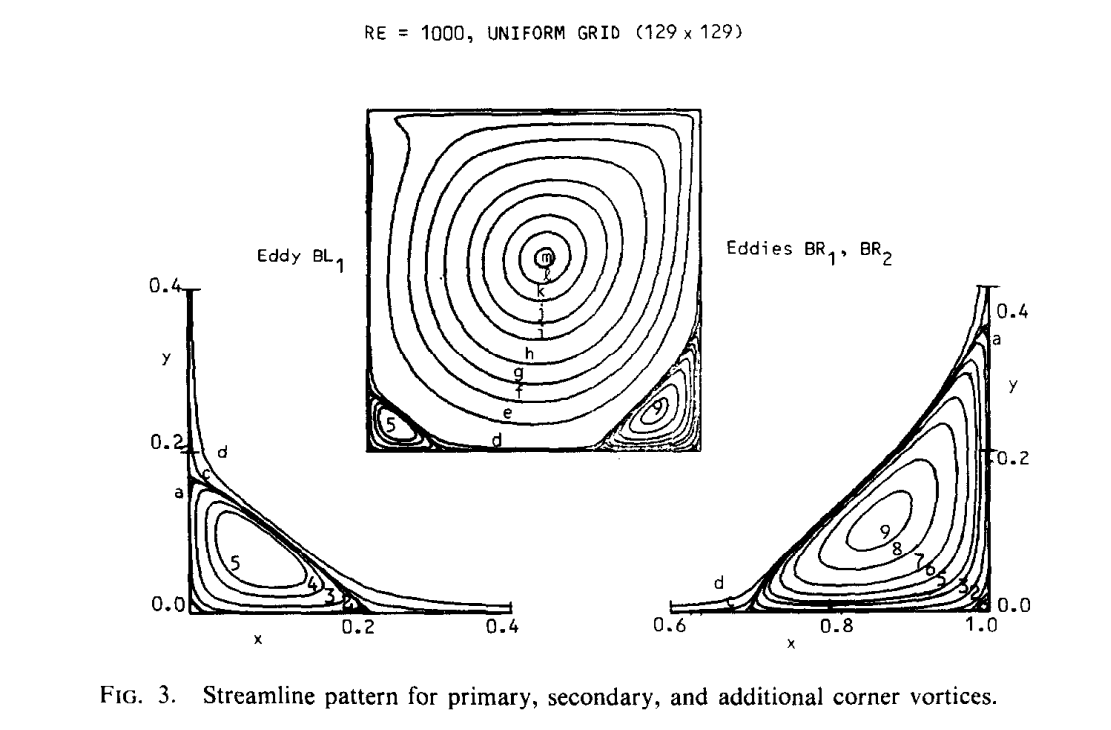
\includegraphics[width=.9\textwidth]{./img/ghia_solution_Re1000.png}
    \caption{Ghia's solution for the lid-driven cavity flow at $Re = 1000$.}
    \label{fig:ghia_solution}
\end{figure}

\begin{figure}[H]
    \centering
    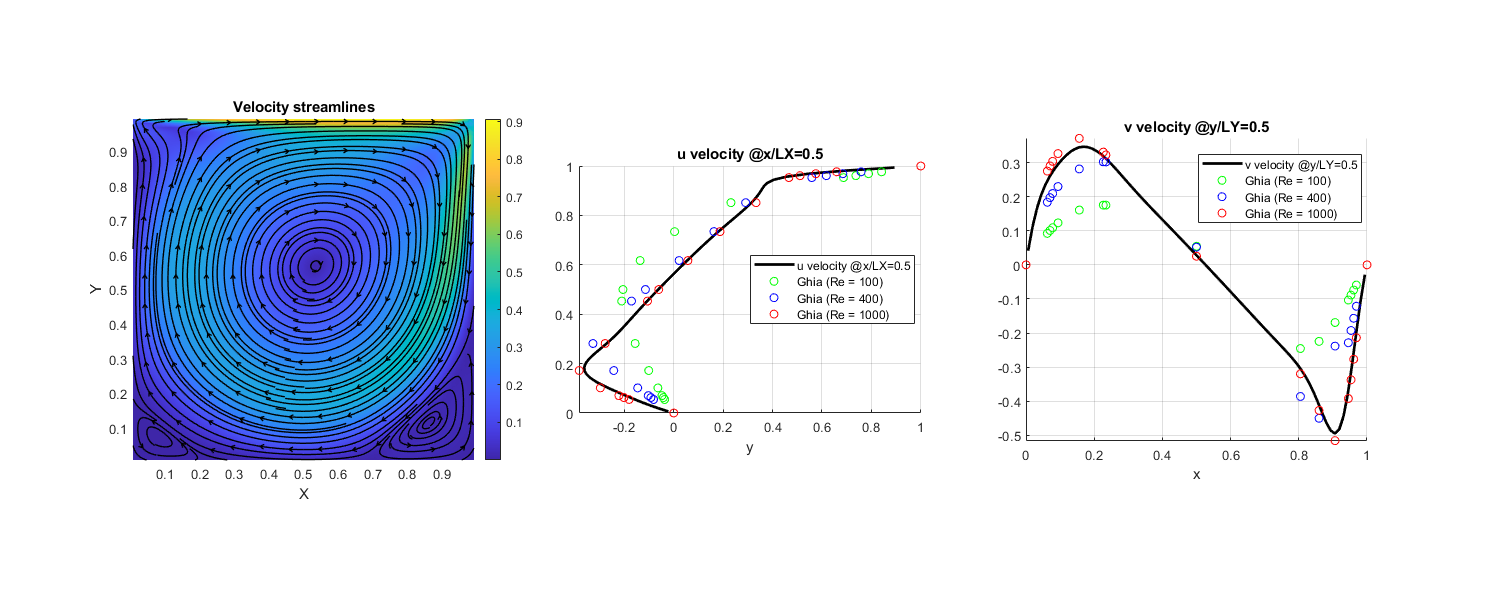
\includegraphics[width=\textwidth]{img/New/SCGS_80x80_008_QUICK.png}
    \caption{SCGS, $80\times80$ mesh, $Re=1000$, $URF_{u,v}=0.08$, QUICK and Second Order schemes for convection and diffusion. Convergence criteria: $10^{-5}$. Iterations: $5000$, last residual: $0.003421$.}
    \label{fig:SCGS_80x80_008_QUICK}
\end{figure}

\begin{figure}[H]
    \centering
    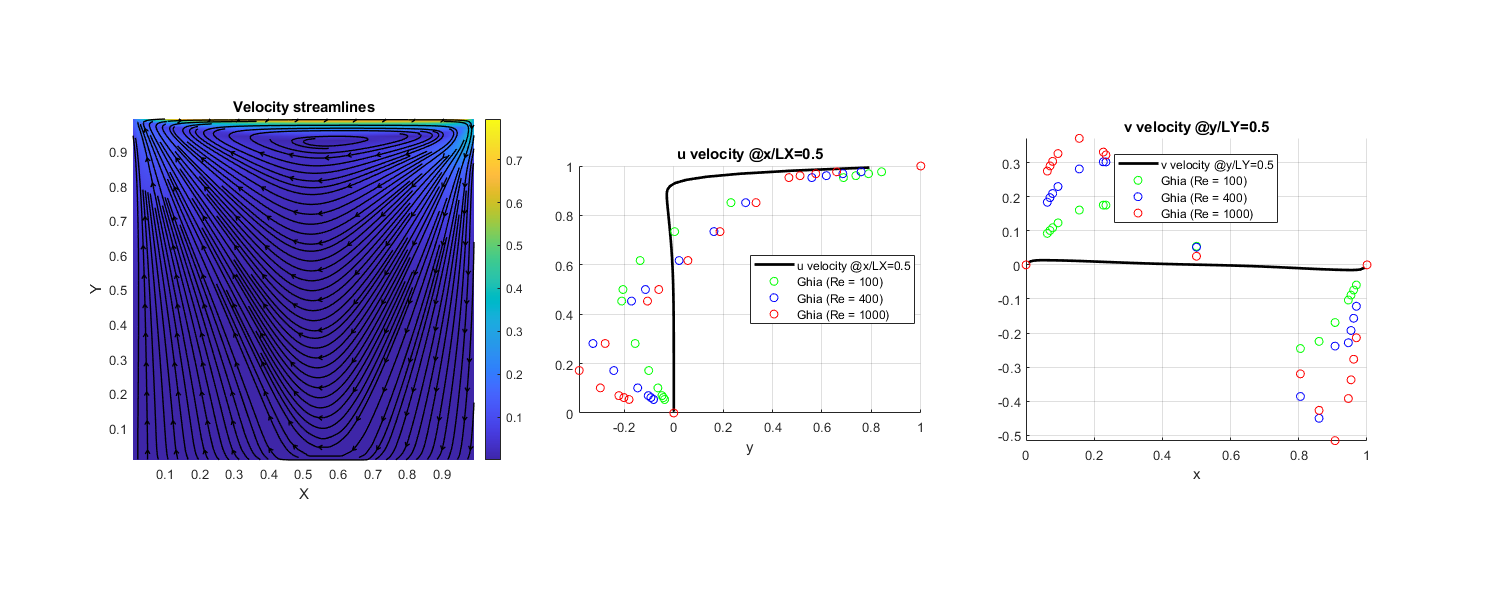
\includegraphics[width=\textwidth]{img/New/50_SIMPLE_80x80_008_003_QUICK.png}
    \caption{SIMPLE, $80\times80$ mesh, $Re=1000$, $URF_{u,v}=0.08$, $URF_p=0.03$, QUICK and Second Order schemes for convection and diffusion. Convergence criteria: $10^{-5}$. Iterations: $50$, last residual: $0.001937$.}
    \label{fig:50_SIMPLE_80x80_008_003_QUICK}
\end{figure}

\begin{figure}[H]
    \centering
    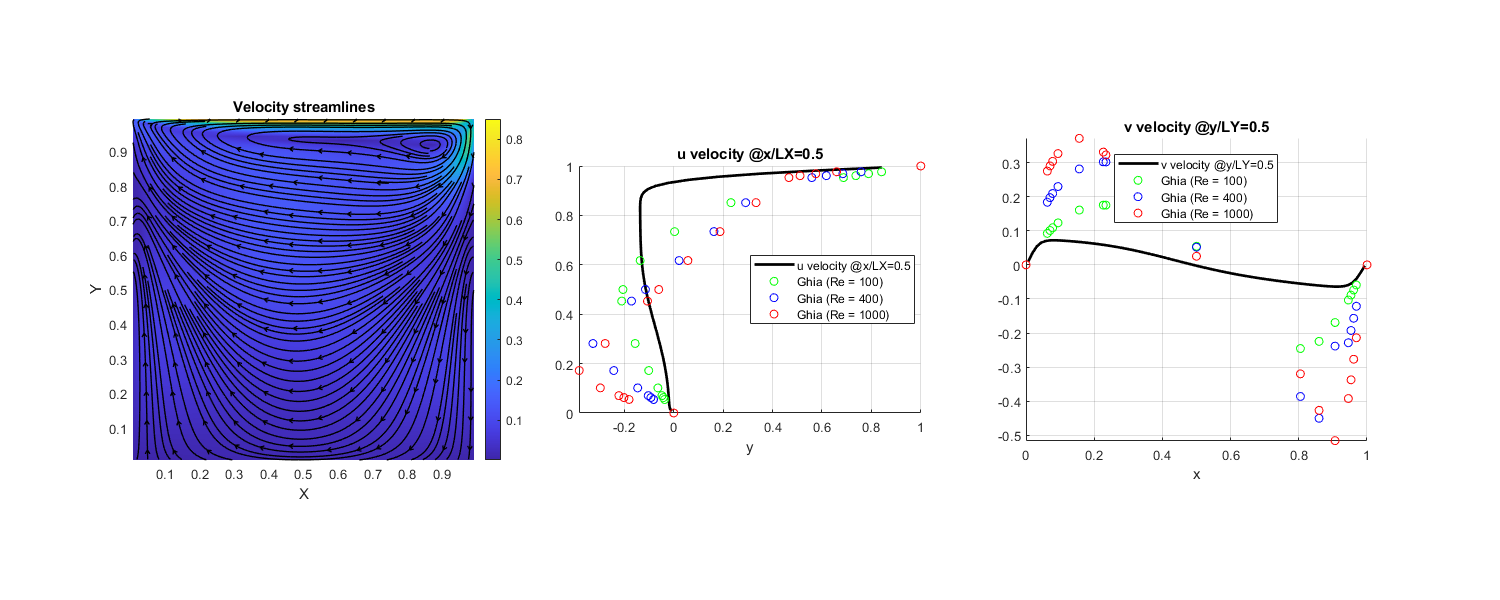
\includegraphics[width=\textwidth]{img/New/100_SIMPLE_80x80_008_003_QUICK.png}
    \caption{SIMPLE, $80\times80$ mesh, $Re=1000$, $URF_{u,v}=0.08$, $URF_p=0.03$, QUICK and Second Order schemes for convection and diffusion. Convergence criteria: $10^{-5}$. Iterations: $100$, last residual: $0.000574$.}
    \label{fig:100_SIMPLE_80x80_008_003_QUICK}
\end{figure}

\begin{figure}[H]
    \centering
    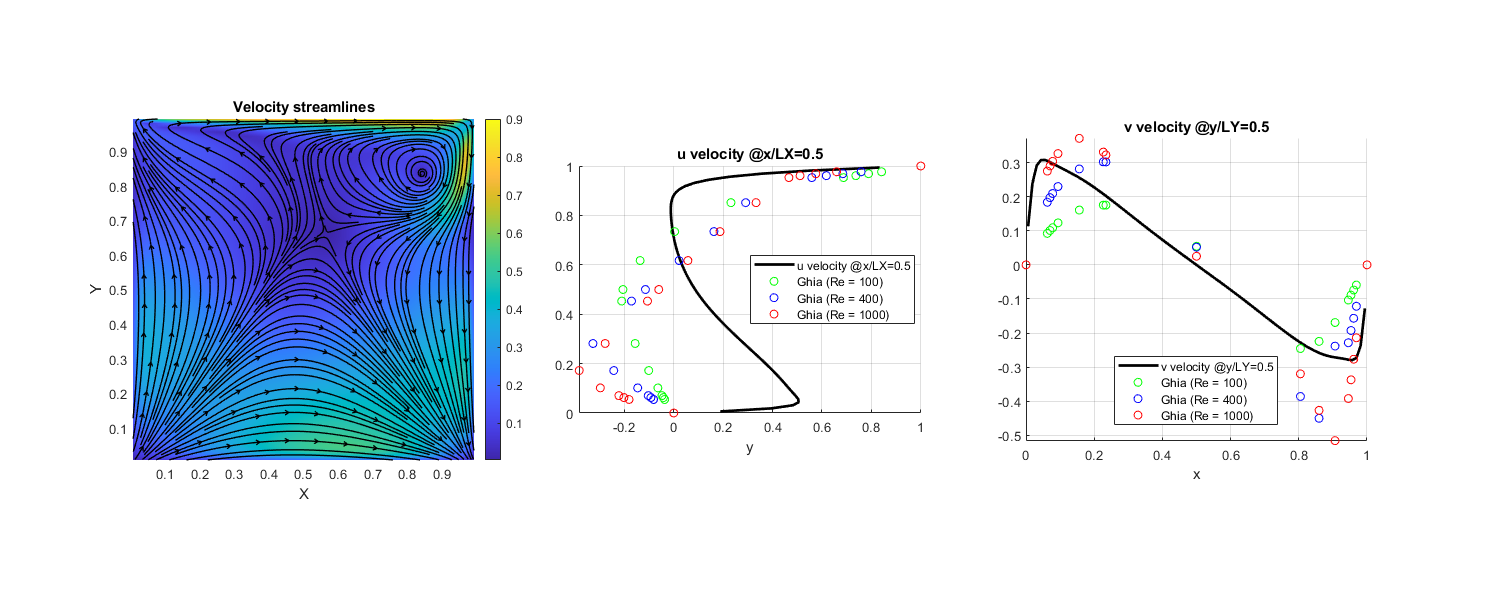
\includegraphics[width=\textwidth]{img/New/200_SIMPLE_80x80_008_003_QUICK.png}
    \caption{SIMPLE, $80\times80$ mesh, $Re=1000$, $URF_{u,v}=0.08$, $URF_p=0.03$, QUICK and Second Order schemes for convection and diffusion. Convergence criteria: $10^{-5}$. Iterations: $200$, last residual: $0.001514$.}
    \label{fig:200_SIMPLE_80x80_008_003_QUICK}
\end{figure}

While the SCGS algorithm at least for given conditions seems to converge even if with excessive number of iterations, the SIMPLE algorithm diverges at iteration $354$, when the states of the system force the overflows of the variables.